%=========================================================================
% sec-intro
%=========================================================================

\section{Introduction}
\label{sec-intro}

In this report, we explore parallelization strategies for the
Floyd-Warshall algorithm for finding the shortest paths between all nodes
in a graph. We start by profiling the naive implementation of the code in
order to identify bottlenecks as well as build our intuition for
developing a relatively accurate performance model. This information is
used to guide the parallelization of the code for both the compute nodes
(i.e., Intel Xeon E5-2620) and the accelerator boards (i.e., Intel Xeon
Phi 5110P) on the Totient cluster. We further implement and evaluate
several optimizations for tuning the parallel code.

%=========================================================================
% fig-intro-dummy.tex
%=========================================================================

\begin{figure}[h]

  \centering
  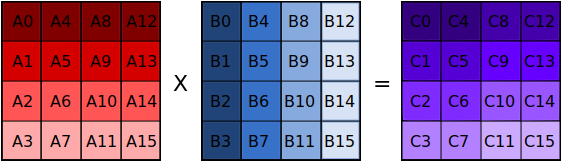
\includegraphics[width=0.7\tw]{fig-intro-dgemm.svg.pdf}

  \caption{\textbf{Dummy Example Image --}
    Lorem ipsum dolor sit amet, consectetur adipiscing elit. Donec
    condimentum rutrum sapien, a fermentum arcu rhoncus non. Aenean
    condimentum ligula sit amet dictum rhoncus. Etiam et justo risus. Sed
    luctus justo ipsum, sit amet sagittis elit porta quis. In placerat mi
    ut scelerisque commodo. Cras sed congue justo. }

  \label{fig-intro-dummy}

\end{figure}

